\documentclass[12pt]{article}

% ---------- Encoding & Fonts ----------
\usepackage[utf8]{inputenc}
\usepackage{amsmath, amssymb, amsfonts, mathtools, bm}
\usepackage{amsthm}
% ---------- Page Layout ----------
\usepackage[a4paper, margin=1in]{geometry}
\usepackage{setspace}
\onehalfspacing
% \usepackage{soul}   % (unused; enable only if you need \hl highlighting)

% ---------- Header/Footer ----------
\usepackage{fancyhdr}
\setlength{\headheight}{14.5pt}
\pagestyle{fancy}
\fancyhf{}
\rhead{Mechatronic Systems}
\lhead{362-2-5401}
\cfoot{\thepage}
\renewcommand{\refname}{Bibliography}

% ---------- Graphics ----------
\usepackage{graphicx}
\graphicspath{{./figures/}{./figs/}}
\usepackage{float}
\usepackage[font=footnotesize]{caption}

% ---------- Listings ----------
\usepackage{listings}
\usepackage{xcolor}
\lstset{
    language=Python,
    basicstyle=\ttfamily\small,
    keywordstyle=\color{blue},
    stringstyle=\color{orange},
    commentstyle=\color{gray},
    numbers=left,
    numberstyle=\tiny\color{gray},
    backgroundcolor=\color{gray!10},
    frame=single,
    rulecolor=\color{gray},
    framerule=0.8pt,
    xleftmargin=1em,
    xrightmargin=1em,
    aboveskip=1em,
    belowskip=1em,
    breaklines=true,
    tabsize=4,
    showstringspaces=false
}
\usepackage{tikz}
\usetikzlibrary{arrows.meta, calc}

\usepackage{titlesec}
\usepackage{booktabs}
\usepackage{array}

\titlespacing*{\subsection}{1.5em}{1.0em}{0.5em}
\titlespacing*{\subsubsection}{2.0em}{1.0em}{0.5em}
\titlelabel{\thetitle.\quad}

% ---------- Hyperlinks ----------
\usepackage{hyperref}

\begin{document}
\begin{titlepage}
    \centering
\includegraphics[width=0.2\textwidth]{figures/bgu.png}\\
        {\fontsize{24}{28}\selectfont Ben-Gurion University of the Negev}\\
    \vspace*{1cm}
{\fontsize{20}{22}\selectfont \bfseries
Nonlinear Adaptive Control of a\\
Mechatronic System\par}
    \vspace{0.1cm}
   \vspace{1.6cm}

    {\Large Tmair Basson \quad Omri Butnaru\par}
    \vspace{0.5cm}
    {\large 318918745 \quad 206340069\par}

    \vspace{2.5cm}

    {\large Lecturers: Shai Arogeti \par}
    \vspace{0.3cm}
    \vspace{0.3cm}
    {\large Ben-Gurion University of the Negev\par}

    \vfill

    {\large June 12, 2026\par}

\end{titlepage}


% ---------------------- TOC ----------------------
\newpage
\tableofcontents
\newpage


% =====================================================================
\section{The Nonlinear Process and Its Model}

\subsection{Physical System}

\noindent The chosen process is a horizontally moving mass connected to a wall through three parallel mechanical elements and driven by an actuator. The benchmark mass--spring--damper with a hardening (cubic) spring is taken from Slotine and Li, \textit{Applied Nonlinear Control} (Prentice Hall, 1991, p.~71), where it appears as a canonical example of a nonlinear mechanical plant. The reference example is second order; to satisfy the assignment requirement of order \(n \geq 3\) we retain the cubic spring nonlinearity and additionally model the actuator as a genuine first-order dynamic element rather than an ideal force source. The added actuator state raises the system order to three.

\begin{figure}[H]
    \centering
    \includegraphics[width=0.95\textwidth]{figs/schematic.png}
    \caption{Physical system (left) and free-body diagram of the mass (right).}
    \label{fig:schematic}
\end{figure}

\noindent The elements acting on the mass are a linear spring of stiffness \(k\), a viscous damper of coefficient \(b\), a nonlinear (cubic) spring producing the restoring force \(\alpha x^3\), and the actuator force \(F(t)\). Summing forces along the direction of motion \(x(t)\) and applying Newton's second law gives the mechanical subsystem:
\[
\boxed{
m\,\ddot{x}(t) + b\,\dot{x}(t) + k\,x(t) + \alpha\,x^3(t) = F(t)
}
\]

\noindent This second-order equation describes the plant if the actuator were ideal, i.e.\ if it produced the commanded force instantaneously. That assumption is relaxed next.

\subsection{The Actuator Model and Its Physical Meaning}

\noindent A real actuator (electric, hydraulic, or pneumatic) cannot deliver a step change of force instantaneously: inductance, fluid compressibility, valve dynamics, or amplifier bandwidth all introduce lag. The simplest faithful representation of this lag is a first-order system relating the commanded input \(u(t)\) to the delivered force \(F(t)\):
\[
\boxed{
\tau\,\dot{F}(t) + F(t) = u(t)
}
\]

\noindent Here \(u(t)\) is the controller command and \(\tau\) is the actuator time constant. The physical meaning is transparent if we hold the command constant at \(u(t)=u_0\) from rest. Solving the first-order ODE gives:
\[
F(t) = u_0\left(1 - e^{-t/\tau}\right).
\]

\noindent The force rises exponentially toward the commanded value, reaching about \(63\%\) of \(u_0\) after one time constant \(\tau\) and approximately \(95\%\) after \(3\tau\). The actuator therefore \textbf{follows} the command with a finite response speed set by \(\tau\), rather than reproducing it instantly. As \(\tau \to 0\) the actuator becomes ideal (\(F \to u\)) and the system collapses back to the original second-order plant. A non-zero \(\tau\) is what gives the combined system its third dynamic state.

\subsection{Eliminating \texorpdfstring{$F(t)$}{F(t)}: the Combined Third-Order Model}

\noindent To obtain a single input--output equation we eliminate the internal force \(F(t)\). From the mechanical subsystem the force is:
\[
F(t) = m\,\ddot{x} + b\,\dot{x} + k\,x + \alpha\,x^3.
\]

\noindent Differentiating once with respect to time:
\[
\dot{F}(t) = m\,\dddot{x} + b\,\ddot{x} + k\,\dot{x} + 3\alpha\,x^2\dot{x}.
\]

\noindent Substituting both \(F(t)\) and its derivative into the actuator relation \(\tau\dot{F} + F = u\) and collecting terms by derivative order yields the combined third-order nonlinear differential equation:
\[
\boxed{
\tau m\dddot{x}(t)+
(\tau b+m)\ddot{x}(t)+(\tau k+b)\dot{x}(t)+kx(t)+3\tau\alpha x^2(t)\dot{x}(t)+\alpha x^3(t)=u(t).
}
\]

\noindent This is the plant the controller must handle. It is genuinely third order and contains two nonlinear terms: the cubic restoring term \(\alpha x^3\) and the mixed term \(3\tau\alpha x^2\dot{x}\) produced by differentiating the cubic spring through the actuator dynamics.

\subsection{State-Space Representation}

\noindent For simulation it is convenient to keep the physical states rather than the input--output form. Choosing \(x_1(t)= x(t)\) (position), \(x_2(t) = \dot{x}(t)\), and \(x_3(t) = F(t)\) (actuator force) gives the first-order system:
\[
\boxed{
\begin{aligned}
\dot{x}_1(t) &= x_2(t),\\
\dot{x}_2(t) &= \frac{1}{m}\left(x_3(t) - b x_2(t) - k x_1(t) - \alpha x_1^3(t)\right),\\
\dot{x}_3 &= \frac{1}{\tau}\left(u(t) - x_3(t)\right).
\end{aligned}
}
\]

\noindent The structure makes the order explicit:
\begin{itemize}
    \item The mechanical mass--spring--damper subsystem contributes two states (position \(x_1\) and velocity \(x_2\)) --- it is second order on its own.
    \item The actuator contributes one additional first-order state (the force \(x_3\)), whose dynamics are governed by the time constant \(\tau\).
    \item The combined actuator-plant system therefore has \textbf{three} states and is \textbf{third order}, satisfying \(n \geq 3\).
\end{itemize}

\subsection{Casting the Plant into the Assignment Model Form}
\noindent The third-order model is
\[
\tau m\dddot{x}(t)+(\tau b+m)\ddot{x}(t)+(\tau k+b)\dot{x}(t)+kx(t)+3\tau\alpha x^2(t)\dot{x}(t)+\alpha x^3(t)=u(t).
\]
\noindent The assignment requires the model to fit the general structure:
\[
y^{(n)}(t) + \sum_{i=1}^{n}\left[a_i\,y^{(n-i)}(t) + b_i\,f_i\!\left(y^{(n-i)}(t)\right)\right] = c\,u(t).
\]

\noindent Dividing the third-order model by the leading coefficient \(\tau m\) and writing \(y(t) \equiv x(t)\), \(n = 3\), the normalized plant is:
\[
\dddot{y}(t)
+
\frac{\tau b+m}{\tau m}\ddot{y}(t)
+
\frac{\tau k+b}{\tau m}\dot{y}(t)
+
\frac{k}{\tau m}y(t)
+
\frac{3\alpha}{m}y^2(t)\dot{y}(t)
+
\frac{\alpha}{\tau m}y^3(t)
=
\frac{1}{\tau m}u(t).
\]

\noindent This matches the assignment form with \(n=3\):
\[
\boxed{
y^{(3)}(t)
+
a_1 \ddot{y}(t)
+
a_2 \dot{y}(t)
+
a_3 y(t)
+
b_1 f_1(y,\dot{y})
+
b_2 f_2(y)
=
c\,u(t)
}
\]

\noindent where
\[
a_1=\frac{\tau b+m}{\tau m}, \quad
a_2=\frac{\tau k+b}{\tau m}, \quad
a_3=\frac{k}{\tau m},
\]
\[
b_1=\frac{3\alpha}{m}, \quad
b_2=\frac{\alpha}{\tau m},  \quad
c=\frac{1}{\tau m},
\]
\noindent and the nonlinear functions are
\[
f_1(y,\dot{y})=y^2(t)\dot{y}(t),
\qquad
f_2(y)=y^3(t).
\]

\noindent Thus the selected mechatronic process satisfies the homework requirements: it is nonlinear, of order three, and derived from a physically meaningful mass--spring--damper--actuator system.

\subsection{Numerical Parameters}

\noindent The physical parameters are chosen consistently with the
second-order reference example, with an actuator time constant
\(\tau = 0.5\)~s. The resulting normalized coefficients are listed below.

\begin{table}[H]
\centering
\caption{Physical and normalized parameters of the selected process.}
\label{tab:params}
\begin{tabular}{@{}llll@{}}
\toprule
\textbf{Quantity} & \textbf{Symbol} & \textbf{Value} & \textbf{Normalized coefficient} \\
\midrule
Mass              & \(m\)      & 1.0 & \(a_1=(\tau b+m)/(\tau m)=2.5\) \\
Linear damping    & \(b\)      & 0.5 & \(a_2=(\tau k+b)/(\tau m)=3.0\) \\
Linear stiffness  & \(k\)      & 2.0 & \(a_3=k/(\tau m)=4.0\) \\
Cubic stiffness   & \(\alpha\) & 1.0 & \(b_1=3\alpha/m=3.0\) \\
Actuator constant & \(\tau\)   & 0.5 & \(b_2=\alpha/(\tau m)=2.0\) \\
\multicolumn{3}{l}{Input gain \(c=1/(\tau m)\)} & \(c=2.0\) \\
\bottomrule
\end{tabular}
\end{table}


% =====================================================================
\section{Adaptive Controller Design}

\noindent In this section a Model Reference Adaptive Control (MRAC) approach is developed for the selected nonlinear mechatronic system. The objective is to make the plant output \(y(t)\) track the output \(y_m(t)\) of a stable reference model, when only the coefficients \(a_i, b_i\) are unknown (the gain \(c\) is assumed known, as stated in the assignment).

\begin{figure}[H]
    \centering
    \includegraphics[width=0.9\textwidth]{figs/blockdiagram.png}
    \caption{Model-reference adaptive control structure: the reference model, adaptive controller, plant, and adaptation law form one closed system.}
    \label{fig:blockdiagram}
\end{figure}

\noindent The homework assignment considers nonlinear systems of the form
\[
y^{(n)}(t)
+
\sum_{i=1}^{n}
\left[
a_i y^{(n-i)}(t)
+
b_i f_i\!\left(y^{(n-i)}(t)\right)
\right]
=
cu(t),
\]
\noindent where the coefficients \(a_i\) and \(b_i\) are unknown constants and the nonlinear functions \(f_i(\cdot)\) are known. For the selected process the output is \(y(t)=x(t)\), and the normalized third-order model is
\[
y^{(3)}(t)
+
a_1\ddot{y}(t)
+
a_2\dot{y}(t)
+
a_3y(t)
+
b_1y^2(t)\dot{y}(t)
+
b_2y^3(t)
=
cu(t).
\]

\noindent The unknown parameter vector and the regressor vector are
\[
\theta=
\begin{bmatrix}
a_1\\ a_2\\ a_3\\ b_1\\ b_2
\end{bmatrix},
\qquad
\phi(t)=
\begin{bmatrix}
\ddot{y}(t)\\ \dot{y}(t)\\ y(t)\\ y^2(t)\dot{y}(t)\\ y^3(t)
\end{bmatrix}.
\]

\noindent The plant is therefore written compactly as
\[
y^{(3)}(t)+\theta^T\phi(t)=cu(t),
\qquad\text{i.e.}\qquad
y^{(3)}(t)=cu(t)-\theta^T\phi(t).
\]

\noindent Although the system is nonlinear in the output \(y(t)\), it is linear in the unknown parameter vector \(\theta\). This property allows a classical MRAC structure with direct parameter adaptation.

\subsection{Reference Model}

\noindent The desired closed-loop behavior is specified by a stable third-order reference model:
\[
\boxed{
y_m^{(3)}(t)
+
\lambda_2\ddot{y}_m(t)
+
\lambda_1\dot{y}_m(t)
+
\lambda_0y_m(t)
=
\lambda_0r(t)
}
\]
\noindent where \(r(t)\) is the reference input. The coefficients \(\lambda_0,\lambda_1,\lambda_2\) are chosen so that
\[
s^3+\lambda_2s^2+\lambda_1s+\lambda_0
\]
\noindent is Hurwitz; therefore the reference model is asymptotically stable. The factor \(\lambda_0\) on the right-hand side gives unity DC gain, so \(y_m\) tracks a constant \(r\) in steady state. The tracking error is
\[
e(t)=y(t)-y_m(t),
\]
\noindent and the control objective is \(\lim_{t\to\infty} e(t)=0\), i.e.\ \(y(t)\rightarrow y_m(t)\).

\subsection{Filtered Tracking Error}

\noindent To simplify the design and the stability proof, define the filtered tracking error
\[
\boxed{
s(t)=\ddot{e}(t)+\alpha_2\dot{e}(t)+\alpha_1e(t)
}
\]
\noindent where \(\alpha_1>0\) and \(\alpha_2>0\) are chosen so that \(p^2+\alpha_2p+\alpha_1\) is Hurwitz. Differentiating,
\[
\dot{s}(t)=e^{(3)}(t)+\alpha_2\ddot{e}(t)+\alpha_1\dot{e}(t).
\]
\noindent Let \(\lambda>0\) be an additional design constant. Choosing the controller gains
\[
k_2=\alpha_2+\lambda,
\qquad
k_1=\alpha_1+\lambda\alpha_2,
\qquad
k_0=\lambda\alpha_1,
\]
\noindent gives the identity
\[
e^{(3)}+k_2\ddot{e}+k_1\dot{e}+k_0e
=
\dot{s}+\lambda s.
\]

\subsection{Adaptive Control Law}

\noindent Let \(\hat{\theta}(t)=[\hat{a}_1,\hat{a}_2,\hat{a}_3,\hat{b}_1,\hat{b}_2]^T\) be the on-line estimate of \(\theta\), with parameter error \(\tilde{\theta}(t)=\hat{\theta}(t)-\theta\). The adaptive control law is
\[
\boxed{
u(t)=
\frac{1}{c}
\left[
y_m^{(3)}(t)
-
k_2\ddot{e}(t)
-
k_1\dot{e}(t)
-
k_0e(t)
+
\hat{\theta}^T(t)\phi(t)
\right].
}
\]

\noindent Substituting into the plant \(y^{(3)}=cu-\theta^T\phi\) gives
\[
y^{(3)}
=
y_m^{(3)}
-
k_2\ddot{e}
-
k_1\dot{e}
-
k_0e
+
\hat{\theta}^T\phi
-
\theta^T\phi.
\]
\noindent Since \(e^{(3)}=y^{(3)}-y_m^{(3)}\),
\[
e^{(3)}
+
k_2\ddot{e}
+
k_1\dot{e}
+
k_0e
=
\tilde{\theta}^T\phi,
\]
\noindent and using the identity of the previous subsection, the tracking error dynamics become
\[
\boxed{
\dot{s}+\lambda s=\tilde{\theta}^T\phi.
}
\]
\noindent The map from the parametric residual \(\tilde{\theta}^T\phi\) to \(s\) is the stable first-order (SPR) filter \(1/(p+\lambda)\), as required by the MRAC stability argument.

\subsection{Adaptation Law}

\noindent The adaptation law is
\[
\boxed{
\dot{\hat{\theta}}(t)=-\Gamma\phi(t)s(t)
}
\]
\noindent where \(\Gamma=\Gamma^T>0\) is the adaptation gain matrix. For a diagonal \(\Gamma=\text{diag}(\gamma_1,\dots,\gamma_5)\) the laws read explicitly
\[
\dot{\hat{a}}_1=-\gamma_1 s\,\ddot{y},
\quad
\dot{\hat{a}}_2=-\gamma_2 s\,\dot{y},
\quad
\dot{\hat{a}}_3=-\gamma_3 s\,y,
\quad
\dot{\hat{b}}_1=-\gamma_4 s\,y^2\dot{y},
\quad
\dot{\hat{b}}_2=-\gamma_5 s\,y^3.
\]

\subsection{Lyapunov Stability Proof}

\noindent Consider the positive-definite Lyapunov candidate
\[
\boxed{
V(t)=
\frac{1}{2}s^2(t)
+
\frac{1}{2}\tilde{\theta}^T(t)\Gamma^{-1}\tilde{\theta}(t).
}
\]
\noindent Since \(\Gamma>0\), \(\Gamma^{-1}\) is positive definite, so \(V\) is positive definite in \(s\) and \(\tilde{\theta}\). Its derivative is
\[
\dot{V}
=
s\dot{s}
+
\tilde{\theta}^T\Gamma^{-1}\dot{\tilde{\theta}}.
\]
\noindent The true parameters are constant, so \(\dot{\tilde{\theta}}=\dot{\hat{\theta}}\). Using \(\dot{s}=-\lambda s+\tilde{\theta}^T\phi\) and \(\dot{\hat{\theta}}=-\Gamma\phi s\),
\[
\dot{V}
=
s\!\left(-\lambda s+\tilde{\theta}^T\phi\right)
+
\tilde{\theta}^T\Gamma^{-1}\!\left(-\Gamma\phi s\right)
=
-\lambda s^2
+
s\tilde{\theta}^T\phi
-
\tilde{\theta}^T\phi\, s.
\]
\noindent The scalars \(s\tilde{\theta}^T\phi\) and \(\tilde{\theta}^T\phi\,s\) are equal and cancel, leaving
\[
\boxed{
\dot{V}=-\lambda s^2\leq 0.
}
\]
\noindent Hence \(V\) is non-increasing and bounded below, so \(s\) and \(\tilde{\theta}\) are bounded and \(s\in L_2\). Under the standard boundedness assumptions, Barbalat's lemma gives \(s(t)\rightarrow 0\) as \(t\rightarrow\infty\). Because \(s=\ddot{e}+\alpha_2\dot{e}+\alpha_1e\) with \(p^2+\alpha_2p+\alpha_1\) Hurwitz, \(s\rightarrow0\) implies
\[
\boxed{
e(t)\rightarrow 0
\quad\Longrightarrow\quad
y(t)\rightarrow y_m(t),
}
\]
\noindent which proves asymptotic tracking. The adaptive law guarantees tracking convergence (\(e\to0\)); convergence of the estimated parameters to their true physical values is not guaranteed unless a persistent-excitation condition holds.


% =====================================================================
\section{Nominal Control with Known Parameters (Simulation)}

\noindent In this section the nominal control signal is derived under the assumption that all plant parameters are known. This case serves as the benchmark for the adaptive controller of Section~4. The normalized plant is \(y^{(3)}(t)+\theta^T\phi(t)=cu(t)\), i.e.\ \(y^{(3)}(t)=cu(t)-\theta^T\phi(t)\).

\subsection{Nominal Control Law}

\noindent Assuming all parameters known, the nominal control law is obtained from the adaptive law of Section~2 by replacing \(\hat{\theta}\) with the true \(\theta\):
\[
\boxed{
u_{\text{nom}}(t)=
\frac{1}{c}
\left[
y_m^{(3)}(t)
-
k_2\ddot{e}(t)
-
k_1\dot{e}(t)
-
k_0e(t)
+
\theta^T\phi(t)
\right].
}
\]
\noindent Here \(e(t)=y(t)-y_m(t)\) and \(y_m(t)\) is generated by the reference model. The gains \(k_2=\alpha_2+\lambda\), \(k_1=\alpha_1+\lambda\alpha_2\), \(k_0=\lambda\alpha_1\) place the error polynomial \(s^3+k_2s^2+k_1s+k_0\) as Hurwitz.

\subsection{Closed-Loop Error Dynamics}

\noindent Substituting the nominal law into the plant, the known nonlinear terms cancel exactly (\(\theta^T\phi-\theta^T\phi=0\)):
\[
y^{(3)}-y_m^{(3)}
=
-k_2\ddot{e}-k_1\dot{e}-k_0e,
\]
\noindent and since \(e^{(3)}=y^{(3)}-y_m^{(3)}\),
\[
\boxed{
e^{(3)}
+
k_2\ddot{e}
+
k_1\dot{e}
+
k_0e
=
0.
}
\]
\noindent With the polynomial Hurwitz, the tracking error converges asymptotically to zero and \(y(t)\rightarrow y_m(t)\).

\subsection{Design Values}

\noindent The reference model is chosen as a triple real pole at \(p=2.5\)~rad/s, giving
\[
\lambda_2 = 3p = 7.5,\qquad
\lambda_1 = 3p^2 = 18.75,\qquad
\lambda_0 = p^3 = 15.625.
\]
\noindent The filtered-error and controller-gain constants are \(\alpha_1=6\), \(\alpha_2=5\), \(\lambda=5\), giving \(k_2=10\), \(k_1=31\), \(k_0=30\). This pole placement is fast enough for good tracking yet compatible with the digital sampling rates used in Sections~5--6.

\begin{figure}[H]
    \centering
    \includegraphics[width=0.7\textwidth]{figs/refmodel.png}
    \caption{Step response of the third-order reference model; smooth, well-damped, unity steady-state gain.}
    \label{fig:refmodel}
\end{figure}

\subsection{Simulation Model and Implementation}

\noindent For the continuous-time simulation the normalized plant is implemented in companion form with \(x_1=y\), \(x_2=\dot{y}\), \(x_3=\ddot{y}\):
\[
\dot{x}_1=x_2,\qquad
\dot{x}_2=x_3,\qquad
\dot{x}_3
=
cu
-
a_1x_3
-
a_2x_2
-
a_3x_1
-
b_1x_1^2x_2
-
b_2x_1^3.
\]
\noindent The reference model is implemented similarly with states \(z_1=y_m\), \(z_2=\dot{y}_m\), \(z_3=\ddot{y}_m\) and \(\dot{z}_3=-\lambda_2z_3-\lambda_1z_2-\lambda_0z_1+\lambda_0r\). At each step the error variables \(e=x_1-z_1\), \(\dot{e}=x_2-z_2\), \(\ddot{e}=x_3-z_3\) are formed, the control \(u_{\text{nom}}\) is computed, and both systems are advanced by explicit Euler integration (\(dt=1\)~ms). The core routine is listed below.

\begin{lstlisting}[caption={Continuous-time closed loop (nominal and adaptive).}, label={lst:cont}]
def simulate_continuous(T=12.0, dt=1e-3, adaptive=False, gamma=5.0, r_amp=1.0):
    n = int(T / dt); t = np.arange(n) * dt
    r = r_amp * np.ones(n)
    x1 = x2 = x3 = 0.0          # plant states: y, y', y''
    z1 = z2 = z3 = 0.0          # reference model states
    th = THETA.copy() if not adaptive else np.zeros(5)
    Y = np.zeros(n); YM = np.zeros(n); E = np.zeros(n); U = np.zeros(n)
    TH = np.zeros((n, 5))
    for i in range(n):
        z3dot = lam0*r[i] - lam2*z3 - lam1*z2 - lam0*z1   # reference model
        e, ed, edd = x1 - z1, x2 - z2, x3 - z3            # tracking error
        s = edd + alpha2*ed + alpha1*e                    # filtered error
        phi = phi_vec(x1, x2, x3)                         # regressor [y'',y',y,y^2 y',y^3]
        u = (1.0/c) * (z3dot - k2*edd - k1*ed - k0*e + th @ phi)
        Y[i], YM[i], E[i], U[i], TH[i] = x1, z1, e, u, th
        x3dot = c*u - THETA @ phi                         # true plant: y'''=c u - theta^T phi
        x1 += x2*dt; x2 += x3*dt; x3 += x3dot*dt          # integrate plant
        z1 += z2*dt; z2 += z3*dt; z3 += z3dot*dt          # integrate reference
        if adaptive:
            th = th - gamma * phi * s * dt                # adaptation law
    return dict(t=t, y=Y, ym=YM, e=E, u=U, th=TH)
\end{lstlisting}

\subsection{Simulation Results}

\noindent Without any controller, the open-loop plant driven by a constant command oscillates and fails to track the reference (Figure~\ref{fig:openloop}). With the nominal controller, the plant output overlays the reference model and the tracking error is zero to machine precision (Figure~\ref{fig:nominal}); the control signal is smooth and bounded (Figure~\ref{fig:nominal_u}). The controller exactly cancels both nonlinearities, so the closed loop behaves like the well-damped linear reference model.

\begin{figure}[H]
    \centering
    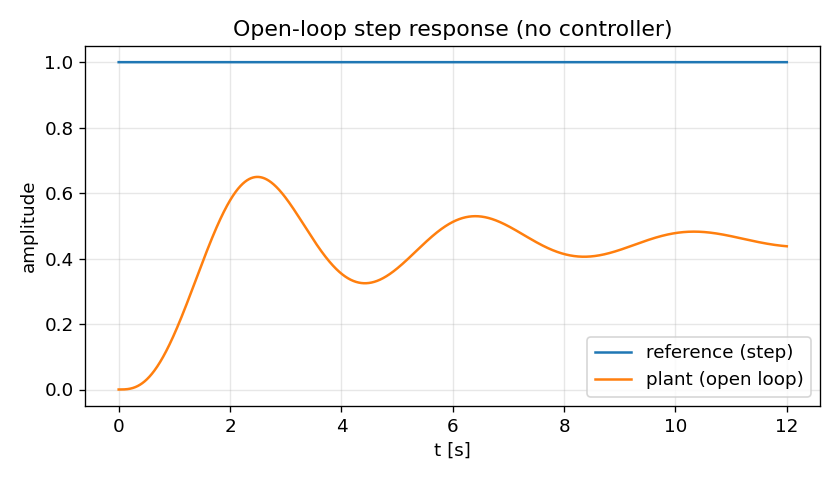
\includegraphics[width=0.7\textwidth]{figures/openloop.png}
    \caption{Open-loop step response (no controller): the plant oscillates and does not track the reference.}
    \label{fig:openloop}
\end{figure}

\begin{figure}[H]
    \centering
    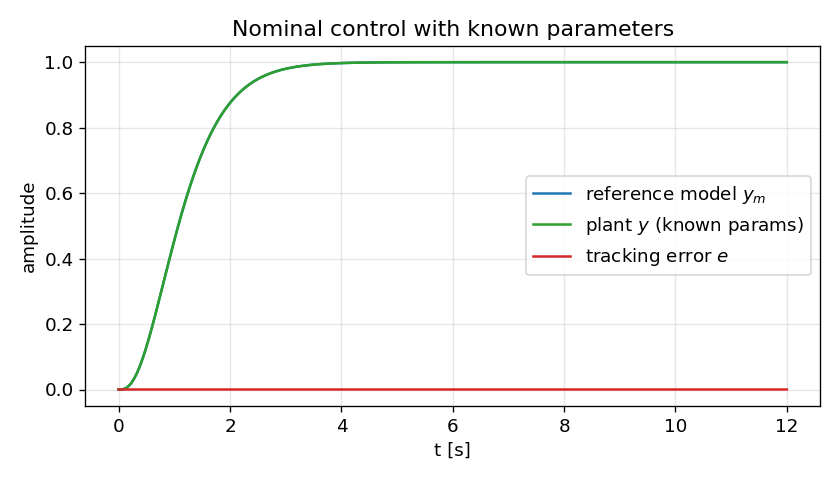
\includegraphics[width=0.7\textwidth]{figures/nominal_tracking.png}
    \caption{Nominal control with known parameters: plant output (green) overlays the reference model (blue); error (red) remains at zero.}
    \label{fig:nominal}
\end{figure}

\begin{figure}[H]
    \centering
    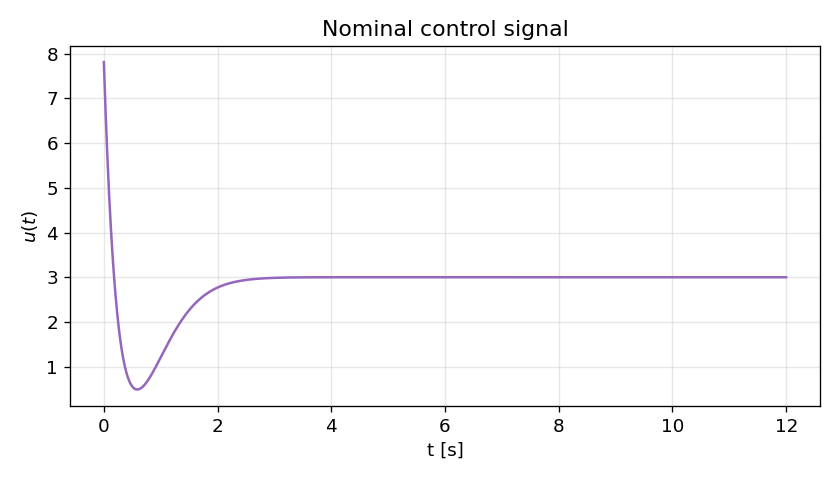
\includegraphics[width=0.7\textwidth]{figures/nominal_u.png}
    \caption{Nominal control signal \(u_{\text{nom}}(t)\): a smooth, bounded effort that cancels the plant dynamics.}
    \label{fig:nominal_u}
\end{figure}


% =====================================================================
\section{Adaptive Control with Unknown Parameters (Simulation)}

\noindent The coefficients \(a_1,a_2,a_3,b_1,b_2\) are now treated as unknown and estimated on-line; the gain \(c\) remains known. The controller uses the same structure as the nominal one but with the estimate \(\hat{\theta}\):
\[
\boxed{
u(t)=
\frac{1}{c}
\left[
y_m^{(3)}(t)
-
k_2\ddot{e}(t)
-
k_1\dot{e}(t)
-
k_0e(t)
+
\hat{\theta}^T(t)\phi(t)
\right],
\qquad
\dot{\hat{\theta}}=-\Gamma\phi s.
}
\]
\noindent For a scalar gain \(\Gamma=\gamma I\) the explicit laws are
\[
\dot{\hat{a}}_1=-\gamma s\,\ddot{y},\:\:
\dot{\hat{a}}_2=-\gamma s\,\dot{y},\:\:
\dot{\hat{a}}_3=-\gamma s\,y,\:\:
\dot{\hat{b}}_1=-\gamma s\,y^2\dot{y},\:\:
\dot{\hat{b}}_2=-\gamma s\,y^3.
\]
\noindent All estimates start from zero initial conditions; the adaptation gain is \(\gamma = 5\), chosen after a short tuning study: large enough for fast convergence, small enough to avoid an over-aggressive transient. The only change relative to Section~3 is the on-line integration of the adaptation law (the \texttt{adaptive=True} branch in Listing~\ref{lst:cont}).

\noindent \textbf{Results.} Even starting with no knowledge of the parameters, the adaptive controller drives the tracking error to zero within the first few seconds and reproduces the known-parameter response after a brief learning transient (Figure~\ref{fig:adaptive}).

\begin{figure}[H]
    \centering
    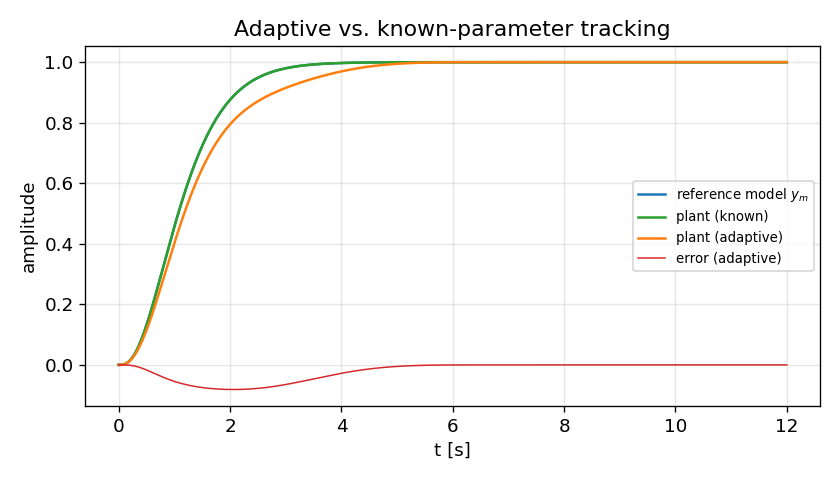
\includegraphics[width=0.78\textwidth]{figures/adaptive_tracking.png}
    \caption{Adaptive vs.\ known-parameter tracking. The adaptive plant (orange) converges to the reference model after a brief transient; both errors decay to zero.}
    \label{fig:adaptive}
\end{figure}

\noindent \textbf{Parameter estimates.} The estimates start at zero and settle to constant values (Figure~\ref{fig:adaptive_params}). They do not converge to the true physical coefficients, and this is expected: a step reference is not persistently exciting, so many parameter combinations achieve the same tracking. The adaptation finds a set of gains that minimizes the tracking error, not necessarily the true plant parameters --- a standard and well-understood feature of MRAC, consistent with the remark closing Section~2.5.

\begin{figure}[H]
    \centering
    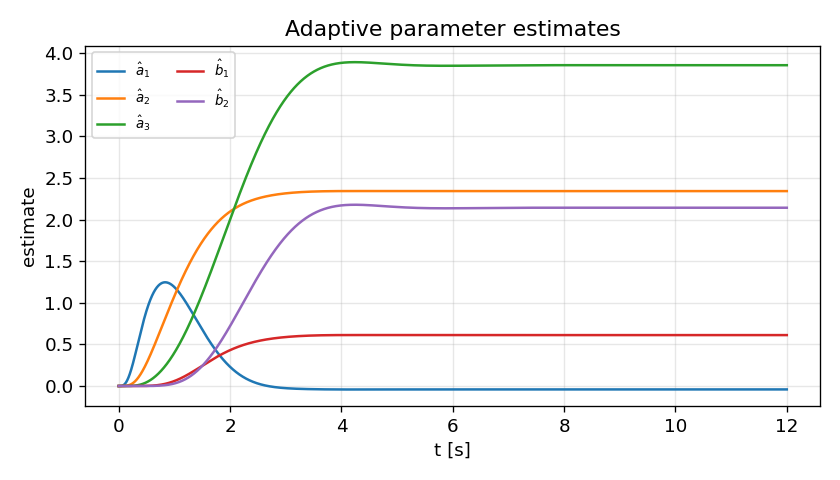
\includegraphics[width=0.78\textwidth]{figures/adaptive_params.png}
    \caption{On-line parameter estimates. They converge to tracking-optimal values, not to the true plant parameters (no persistent excitation under a step input).}
    \label{fig:adaptive_params}
\end{figure}


% =====================================================================
\section{Digital Implementation (Indirect Design)}

\noindent A microcontroller realization requires a discrete-time controller. Using the \textbf{indirect digital design} approach, the continuous controller of Section~2 is designed first and then discretized: derivatives are approximated by differences and the control output is held constant between samples by a zero-order hold (ZOH). The continuous plant keeps evolving in continuous time; only the controller is sampled.

\subsection{Discretization by Difference Equations}

\noindent Derivatives are approximated by backward differences at sampling period \(T\):
\[
\dot{y}(k) \approx \frac{y(k) - y(k-1)}{T}.
\]
\noindent For this relative-degree-three plant, a raw second backward difference amplifies sampling noise so severely that the loop becomes unstable. A robust and standard remedy is the \textbf{filtered (dirty) derivative}: a first-order low-pass applied to each difference, with pole \(1/\tau_d\),
\[
\boxed{
\dot{y}_f(k) = a_f\,\dot{y}_f(k-1) + (1-a_f)\,\frac{y(k)-y(k-1)}{T},
\qquad a_f = \frac{\tau_d}{\tau_d + T},
}
\]
\noindent and similarly for the second derivative. The discrete adaptation law uses the regressor-normalized update
\[
\hat{\theta}(k) = \hat{\theta}(k-1) - \gamma\,\frac{\phi(k)\,s(k)}{1+\phi^{T}\phi}\,T.
\]

\subsection{Zero-Order Hold}

\noindent Between sampling instants the controller cannot issue new commands, so the last computed value is held:
\[
u(t) = u(kT),\qquad kT \leq t < (k+1)T.
\]
\noindent The ZOH converts the discrete command sequence into the piecewise-constant analog signal applied to the actuator; its staircase shape is visible in Figure~\ref{fig:discrete_u}. The discrete closed-loop routine is listed below.

\begin{lstlisting}[caption={Discrete-time controller with ZOH (indirect digital design).}, label={lst:disc}]
def simulate_discrete(Ts, T=12.0, dt_plant=1e-3, adaptive=True, gamma=5.0,
                      tau_d=0.03, use_pid=False, Kp=0.8, Ki=0.1, Kd=3.0, r_amp=1.0):
    n = int(T/dt_plant); t = np.arange(n)*dt_plant
    r = r_amp*np.ones(n); steps = max(1, int(round(Ts/dt_plant)))
    x1 = x2 = x3 = 0.0; z1 = z2 = z3 = 0.0
    th = THETA.copy() if not adaptive else np.zeros(5)
    u_hold = 0.0; integ = 0.0
    y_prev = 0.0; yd_f = 0.0; ydd_f = 0.0; yd_prev = 0.0
    af = tau_d/(tau_d + Ts)
    Y=np.zeros(n); YM=np.zeros(n); E=np.zeros(n); U=np.zeros(n); TH=np.zeros((n,5))
    for i in range(n):
        if i % steps == 0:                                  # sampling instant
            y = x1
            z3dot = lam0*r[i] - lam2*z3 - lam1*z2 - lam0*z1
            raw_yd = (y - y_prev)/Ts                         # filtered derivatives
            yd_f = af*yd_f + (1-af)*raw_yd
            raw_ydd = (yd_f - yd_prev)/Ts
            ydd_f = af*ydd_f + (1-af)*raw_ydd
            yd, ydd = yd_f, ydd_f
            e, ed, edd = y - z1, yd - z2, ydd - z3
            s = edd + alpha2*ed + alpha1*e
            phi = phi_vec(y, yd, ydd)
            u_mrac = (1.0/c)*(z3dot - k2*edd - k1*ed - k0*e + th @ phi)
            if use_pid:
                integ += e*Ts
                u_hold = u_mrac - (Kp*e + Ki*integ + Kd*ed)
            else:
                u_hold = u_mrac
            if adaptive:
                th = th - gamma*phi*s*Ts/(1.0 + phi @ phi)   # discrete adaptation
            y_prev = y; yd_prev = yd_f
        Y[i], YM[i], E[i], U[i], TH[i] = x1, z1, x1 - z1, u_hold, th   # ZOH hold
        x3dot = c*u_hold - THETA @ phi_vec(x1, x2, x3)
        x1 += x2*dt_plant; x2 += x3*dt_plant; x3 += x3dot*dt_plant
        z3d = lam0*r[i] - lam2*z3 - lam1*z2 - lam0*z1
        z1 += z2*dt_plant; z2 += z3*dt_plant; z3 += z3d*dt_plant
    return dict(t=t, y=Y, ym=YM, e=E, u=U, th=TH)
\end{lstlisting}

\subsection{Closed-Loop Results}

\noindent Combining the discrete controller (with ZOH) and the continuous plant, the closed loop tracks the reference model well at \(20\)~Hz, with only a small loss of accuracy relative to the continuous design (tracking RMSE \(\approx 0.048\) versus \(0.035\) continuous). The discrete response shows a small phase lag introduced by the hold but remains stable and accurate (Figure~\ref{fig:discrete}). The on-line estimates converge similarly to the continuous case, slightly slower due to sampling (Figure~\ref{fig:discrete_params}).

\begin{figure}[H]
    \centering
    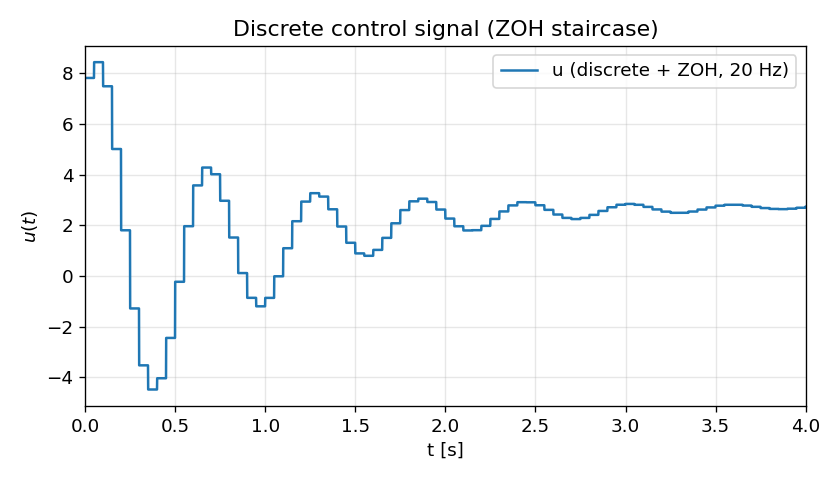
\includegraphics[width=0.7\textwidth]{figures/discrete_u.png}
    \caption{Discrete control signal with ZOH at \(20\)~Hz. The piecewise-constant staircase is the signal applied to the continuous plant.}
    \label{fig:discrete_u}
\end{figure}

\begin{figure}[H]
    \centering
    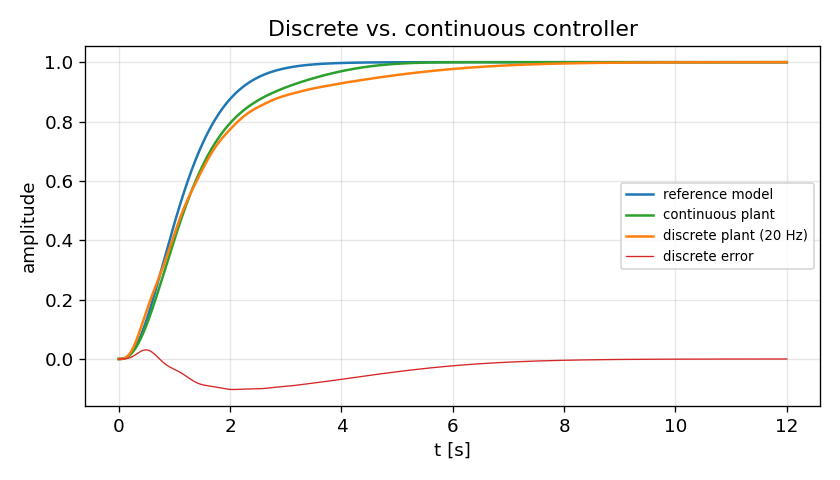
\includegraphics[width=0.78\textwidth]{figures/discrete_tracking.png}
    \caption{Discrete (20~Hz) vs.\ continuous controller. The discrete loop tracks well; the hold adds a small phase lag.}
    \label{fig:discrete}
\end{figure}

\begin{figure}[H]
    \centering
    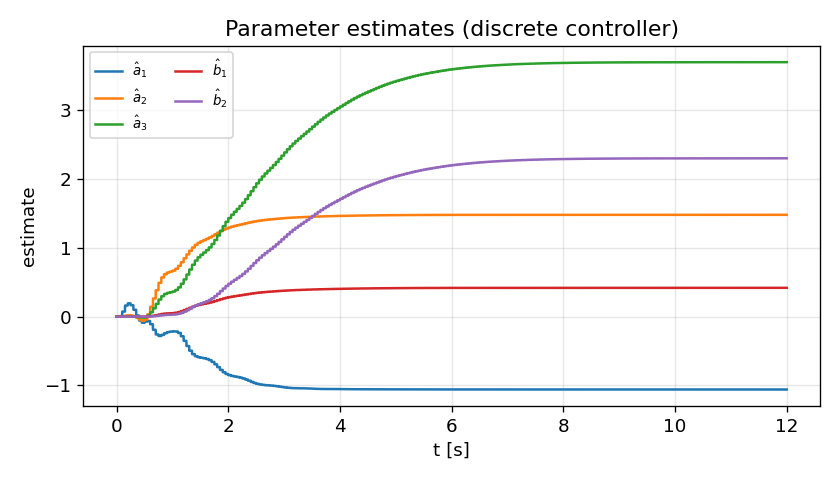
\includegraphics[width=0.78\textwidth]{figures/discrete_params.png}
    \caption{On-line parameter estimates with the discrete controller; convergence is slightly slower than the continuous case due to sampling.}
    \label{fig:discrete_params}
\end{figure}


% =====================================================================
\section{Sampling-Time Effects and a PID Remedy}

\subsection{Performance Degradation with Larger Sampling Time}

\noindent As the sampling period \(T\) increases, two effects worsen the closed loop. First, the ZOH holds each command longer, which is equivalent to an average transport delay of \(T/2\) and therefore adds phase lag. Second, the difference-based derivative estimates become coarser. Both effects erode the stability margin of the relative-degree-three loop. Figure~\ref{fig:sweep} shows a graceful degradation followed by a sharp stability cliff: the tracking RMSE rises gently from \(0.048\) at \(20\)~ms to \(0.053\) at \(65\)~ms, and the loop becomes unstable at \(70\)~ms. The dominant cause is the ZOH delay, which produces phase lag and an amplitude deficit precisely when the reference model is changing fastest (the first \(\sim\!2\)~seconds of the step).

\begin{figure}[H]
    \centering
    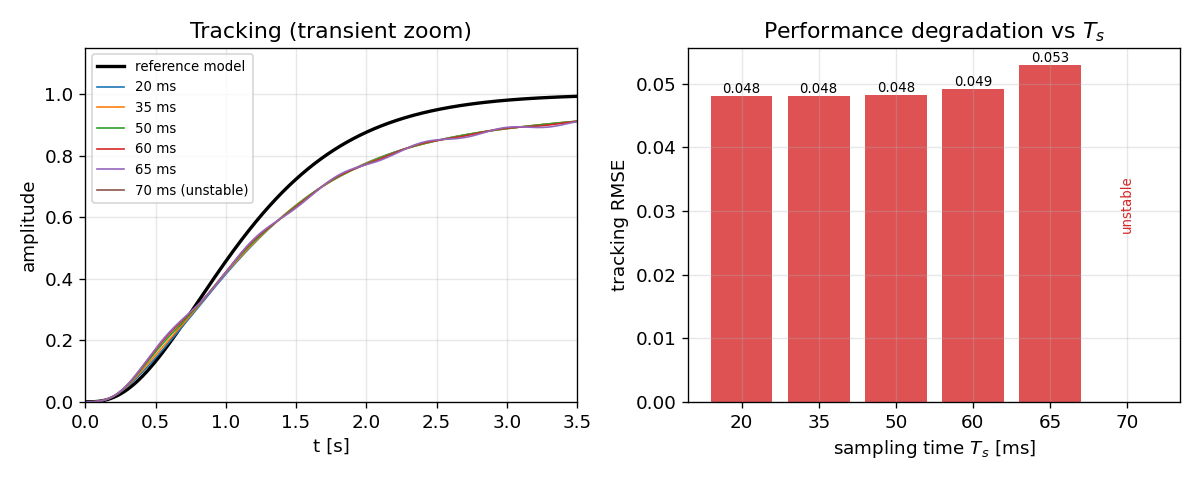
\includegraphics[width=0.95\textwidth]{figures/sampling_sweep.png}
    \caption{Effect of increasing sampling time. Left: transient tracking degrades as \(T_s\) grows. Right: tracking RMSE rises gently up to \(65\)~ms, then the loop becomes unstable at \(70\)~ms.}
    \label{fig:sweep}
\end{figure}

\subsection{Reducing the Degradation: PID Phase-Lead Augmentation}

\noindent To recover the lost performance without raising the sampling rate, a PID compensator is added in parallel with the adaptive controller. The derivative action supplies phase lead that counteracts the ZOH phase lag, while the proportional and integral actions restore amplitude and remove residual error. The total command is
\[
u_{\text{total}} = u_{\text{mrac}} + u_{\text{pid}},
\qquad
u_{\text{pid}} = -\!\left(K_P\,e + K_I\!\int_0^t e\,d\tau + K_D\,\dot{e}\right),
\]
\noindent with \(e=y-y_m\). After calibration the gains were \(K_P=0.8\), \(K_I=0.1\), \(K_D=3.0\). At a coarse \(50\)~ms update, the PID-augmented controller tracks the reference slightly better than the plain discrete MRAC (RMSE \(0.047\) versus \(0.048\)) and produces a smoother transient (Figure~\ref{fig:pid}). The PID component is most active during the initial transient, where it injects the corrective effort needed to compensate the phase lag, and thereafter contributes only mild trimming (Figure~\ref{fig:pid_u}).

\begin{figure}[H]
    \centering
    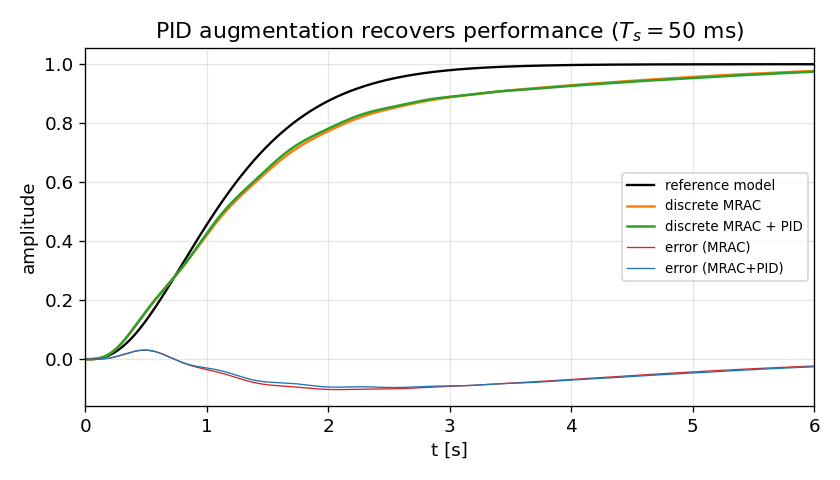
\includegraphics[width=0.78\textwidth]{figures/pid_tracking.png}
    \caption{PID augmentation at \(T_s=50\)~ms. The MRAC+PID response (green) follows the reference model more closely than plain discrete MRAC (orange).}
    \label{fig:pid}
\end{figure}

\begin{figure}[H]
    \centering
    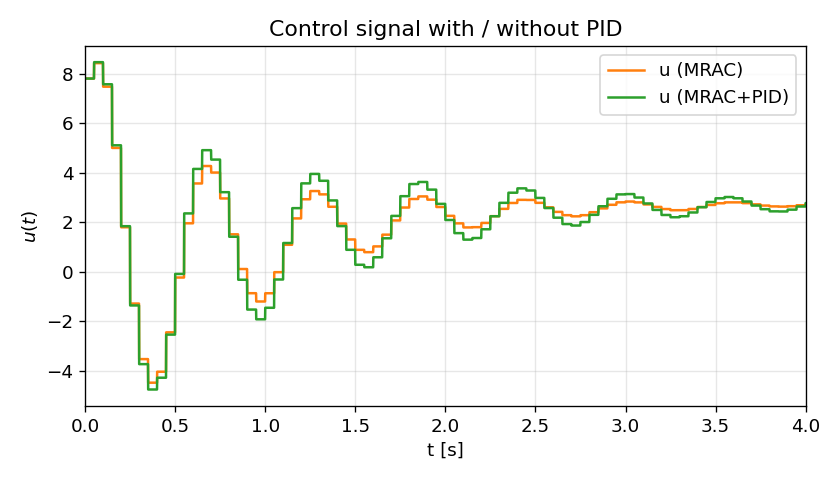
\includegraphics[width=0.7\textwidth]{figures/pid_u.png}
    \caption{Control signals with and without PID. The PID adds an early corrective effort, then settles to gentle trimming.}
    \label{fig:pid_u}
\end{figure}

\subsection{Discussion}

\noindent The experiments confirm the expected digital-control phenomenology: phase lag and reduced stability margin worsen as the sampling period grows, with the ZOH delay as the principal cause. The degradation is gradual until the loop nears its stability boundary, beyond which it deteriorates abruptly. Augmenting the discrete adaptive law with a PID compensator improves performance at a coarse sampling rate by supplying compensating phase lead, at the modest cost of a more aggressive initial control effort. Further improvement is expected from systematic tuning of the PID gains or from redesigning the discrete controller directly in the \(z\)-domain.


% =====================================================================
\begin{thebibliography}{9}
\bibitem{slotine}
J.-J. E. Slotine and W. Li,
\textit{Applied Nonlinear Control},
Prentice Hall, Englewood Cliffs, NJ, 1991
(mass--spring--damper with nonlinear spring, p.~71).
\end{thebibliography}


\end{document}
